\documentclass[conference]{IEEEtran}
\IEEEoverridecommandlockouts
% The preceding line is only needed to identify funding in the first footnote. If that is unneeded, please comment it out.
\usepackage{cite}
\usepackage{amsmath,amssymb,amsfonts}
\usepackage{algorithmic}
\usepackage{graphicx}
\usepackage{textcomp}
\usepackage{xcolor}
\usepackage{multirow}
\usepackage{array}

\def\BibTeX{{\rm B\kern-.05em{\sc i\kern-.025em b}\kern-.08em
    T\kern-.1667em\lower.7ex\hbox{E}\kern-.125emX}}
\begin{document}

\title{Classificação de textos em português utilizando diferentes técnicas de embedding do Word2vec ao GPT\\
}

\author{\IEEEauthorblockN{Thomas Edson Cordeiro dos Santos}
\IEEEauthorblockA{\textit{Programa de Pós-Graduação em Informática - PPGI} \\
\textit{Universidade Federal do Espírito Santo - UFES}\\
Vitória, Brasil \\
thomas.santos@ufes.edu.br}
\and
\IEEEauthorblockN{Wharley Borges Ferreira}
\IEEEauthorblockA{\textit{Programa de Pós-Graduação em Informática - PPGI} \\
\textit{Universidade Federal do Espírito Santo - UFES}\\
Vitória, Brasil \\
wharley.ferreira@edu.ufes.br}
}

\maketitle

\begin{abstract}
Neste trabalho nós comparamos diversos modelos de \textit{embedding} de texto em português brasileiro. A qualidade dos resultados foi avaliada na tarefa de classificação da variável binária conformidade de textos das ordens de manutenção do SAP da indústria de óleo e gás. O modelo que demonstrou melhores resultados foi um Word2vec (Petrovec-O\&G de 100 dimensões) treinado com mais de 85 milhões de tokens de documentos públicos desta indústria. Este modelo obteve um recall de 78 \%, superando até mesmo modelos baseados na arquitetura transformers, que tem apresentado de maneira consistente resultados no estado da arte em tarefas de processamento de linguagem natural.
\end{abstract}

\begin{IEEEkeywords}
português, \textit{embedding}, processamento de linguagem natural, classificação de textos
\end{IEEEkeywords}

\section{Introdução}

  O campo de processamento de linguagem natural (do inglês \textit{Natural Language Processing} - NLP) é uma área da inteligência artificial que tem evoluído rapidamente nos últimos anos. O ChatGPT da OpenAI \cite{NIPS2017_3f5ee243} \cite{Radford2018ImprovingLU} \cite{radford_language_2019} \cite{brown2020language} ganhou as manchetes por apresentar um modelo que consegue "conversar" com o usuário com uma facilidade e fluência nunca vistos antes. Grandes modelos de linguagem (do inglês \textit{Large Language Models} - LLM) proprietários apresentam sistematicamente resultados do estado da arte, porém são muito pesados para rodar localmente, sendo disponibilizados por meio de chamadas de API, que possuem custo associado, depende da confiabilidade do serviço e em alguns casos os dados podem ser usados para treinamento de versões posteriores do modelo, levantando questões sobre sigilo e ética. Outra limitação atual dos modelos baseados em transformers é o tamanho fixo da entrada, o que inviabiliza alguns tipos de análise. O presente trabalho apresenta a avaliação da aplicabilidade de tecnologias para classificação de textos em português em uma base de dados de ordem de manutenção no sistema SAP. Atualmente essa análise é realizada manualmente por diversas pessoas, com uma cobertura em parte das ordens que são geradas a cada mês. A proposta é que esta análise seja realizada automaticamente em todas as ordens e, apenas as ordens mais prováveis de oportunidades de melhorias, sejam avaliadas posteriormente por humanos. Nesta abordagem, seria realizada uma cobertura maior das ordens e o uso do trabalho humano seria otimizado. Essas ordens contêm informações possivelmente sensíveis, dessa forma, os dados devem ser tratados em ambientes seguros. Por esse motivo, os dados só foram tratados através de API privada ou modelos rodando localmente. Um dos objetivos da presente revisão é avaliar se a tecnologia por trás do ChatGPT ou as usadas por seus concorrentes treinados especificamente em português do Brasil \cite{souza2020bertimbau} \cite{Gomes2021} podem ser aplicadas para classificar com eficiência textos escritos nesse idioma. Foi realizada uma revisão sistemática sobre a classificação de textos em português para verificar quais as técnicas mais promissoras. Ao final do trabalho são apresentados os desempenhos obtidos com diferentes técnicas e é observado que técnicas simples, abertas e consolidadas geram resultados competitivos com as tecnologias mais novas e proprietárias.
  Na seção II serão apresentadas as técnicas de \textit{embedding}, na III são apresentados os resultados obtidos com essas técnicas e, por fim, na IV são apresentadas as conclusões.

\section{Ferramentas de embedding de texto utilizadas}

  Para realizar a classificação de textos com uso de modelos de inteligência artificial, é necessário primeiro transformar esses textos em números. Essa tarefa é chamada de embedding e, ao contrário do que pode parecer, não é trivial. A abordagem mais simples para essa conversão é atribuir a cada possível palavra uma dimensão (ou coluna em uma matriz), porém essa abordagem tipicamente gera matrizes esparsas de alta dimensionalidade. Essa abordagem gera inconvenientes chamados de "maldição da dimensionalidade" (do inglês \textit{curse of dimensionality}). Um trabalho de 2003 \cite{bengio2003} introduziu a ideia de aprender uma representação distribuída das palavras que consegue, não só representar de forma compacta e eficiente as entidades, mas também as relações entre esses conceitos. Nessa abordagem, as palavras e sentenças devem ser distribuídas em um espaço multidimensional de forma que sentenças similares possuam localizações similares. Por mais simples que possa parecer, essa modelagem se mostrou extremamente poderosa e permite a construção de um "modelo de mundo" de tokens, que é uma das pedras fundamentais da revolução que o campo de processamento de linguagem natural tem passado nos últimos anos.
  Foi realizado um mapeamento sistemático com vistas a localizar ferramentas de \textit{embedding} utilizadas em trabalhos científicos. Um requisito essencial para a seleção das publicações foi buscar as voltadas ao idioma português, preferencialmente o Brasileiro. Considerando a grande revolução que houve nos últimos anos na área de NLP devido ao advento da arquitetura de transformers \cite{NIPS2017_3f5ee243}, foram pesquisados artigos publicados a partir de 2018.

\subsection{TF-IDF}

  De forma a evitar um viés pelo uso exclusivo de técnicas novas, foi utilizada como referência a codificação de textos por meio de \textit{Term Frequency-Inverse Document Frequency} (TF-IDF), após o que foi realizada a redução de dimensionalidade para 1000 por meio de SVD no que é conhecido como análise semântica latente (do inglês \textit{latent semantic analysis} - LSA).  O pré-processamento de texto consistiu em: conversão para minúsculo, eliminação de linhas com texto em branco, tokenização, remoção de stopwords, stemming após o qual foi criada uma matriz do tipo TF-IDF e realizada uma redução de dimensionalidade com SVD (do inglês \textit{Singular Value Decomposition}).

\subsection{Petrolês}
  
  Um dos trabalhos identificados através da revisão da literatura \cite{Gomes2021} corresponde ao resultado de uma colaboração interinstitucional liderada pelo Centro de Pesquisas e Desenvolvimento da Petrobras (CENPES), em parceria com PUC-Rio, UFRGS e PUC-RS, e visa incentivar pesquisas nas áreas de Processamento de Linguagem Natural e Linguística Computacional aplicadas ao domínio de Óleo e Gás (O\&G).
  O Petrolês (https://petroles.puc-rio.ai/) é um repositório de artefatos de Processamento de Linguagem Natural especializados no domínio de petróleo em Português, e tem como objetivo servir como uma referência para os grupos de pesquisas em inteligência artificial e empresas atuantes nesse domínio. Dentre os artefatos disponíveis livremente no repositório foram utilizados no presente trabalho três modelos de word embedding do tipo Word2vec sendo dois deles, Petrovec-O\&G de 100 e 300 dimensões, treinados unicamente a partir de dados públicos relacionados ao domínio de O\&G (Boletins Técnicos da Petrobras; Teses e Dissertações em assuntos relacionados à indústria de Petróleo; Notas e estudos técnicos da ANP). O terceiro modelo Petrovec-híbrido de 100 dimensões treinado nos mesmos documentos que os modelos O\&G e adicionalmente em um corpus de contexto geral em Português do NILC.

\subsection{BERTimbau}

  Uma ferramenta citada recorrentemente nas publicações foi o BERT (do inglês \textit{Bidirectional Encoder Representations for Transformers}) da Google, em particular uma versão que passou por um \textit{fine-tunning em português}, o BERTimbau \cite{souza2020bertimbau}. Esse modelo foi obtido através da biblioteca transformers do Hugging Face distribuída como padrão no pacote ANACONDA. O nome formal do modelo na biblioteca é o "neuralmind/bert-base-portuguese-cased". Como saída, o BERT gera um tensor contendo um vetor de 768 dimensões para cada token. De forma a obter um \textit{embedding} para toda a sentença, foi realizada a média entre todos os os vetores do tensor, sendo gerada dessa forma apenas um vetor de 768 por sentença. 

\subsection{SBERT}

  Também foi utilizada uma versão modificada do BERT específica para o \textit{embedding} de sentenças, o SBERT \cite{reimers-2019-sentence-bert} com uma versão treinada 15 idiomas e outra treinada em mais de 50 idiomas \cite{reimers-2020-multilingual-sentence-bert}. Como saída esses modelos geram apenas um vetor de 768 dimensões para cada sentença. Os modelos específicos utilizados nas simulações foram o "distiluse-base-multilingual-cased-v1" e o "distiluse-base-multilingual-cased-v2" respectivamente, disponíveis na biblioteca sentence\_transformers.

\subsection{GPT}

  Uma ferramenta de processamento de linguagem natural que ganhou muita atenção recentemente foi o ChatGPT da OpenAI. Em conjunto com os chatbots, a OpenAI disponibiliza as \textit{engines} por trás desses serviços através de APIs. A Petrobras disponibilizou, em parceria com a Microsoft um serviço com algumas das mais poderosas e recentes ferramentas da OpenAI. No caso do trabalho em questão, não foi cogitado usar a API de chat devido ao limite do tamanho de entrada. O conjunto de dados possui milhares de textos com dezenas de milhares de tokens. Foi utilizada, no entanto uma API de segunda geração, que de acordo com a própria OpenAI supera as APIs da primeira geração na maioria das tarefas. No presente trabalho foi utilizada especificamente uma versão interna da engine "text-embedding-ada-002". O serviço recebe uma sentença de até 8191 tokens e devolve um vetor com 1536 dimensões. Existe um trabalho bastante detalhado descrevendo o funcionamento da primeira geração de APIs \cite{neelakantan2022text}, porém a documentação relativa à segunda geração de embeddings é mais escassa, o que reflete uma tendência recente dos produtos oferecidos pela OpenAI desde os grandes investimentos recebidos da Microsoft. 

\section{Resultados}

Foram realizadas simulações com uma amostra de cerca de 2000 ordens. Considerando que a base de dados é desbalanceada (muito mais classe 0 que classe 1), também foram realizadas simulações com data augmentation por meio de SMOTE. A partir dos dados processados para cada técnica de embedding, combinada ou não com SMOTE foram realizadas classificações com três classificadores diferentes, um do tipo Random Forest (RF), Redes Neurais (NN) e XGBoost. As principais métricas para cada uma dessas simulações se encontram listadas na tabela ~\ref{table:resultados}

\begin{table*}[t]
\centering
\caption{Principais resultados das simulações com diferentes métodos de embedding e diferentes classificadores}
\label{table:resultados}
\def\arraystretch{1.2}
\begin{tabular}{lclccccccccc}
\hline
Embedding                          & SMOTE              & Modelo  & TN  & FP & FN & TP & precision & recall & F1 & F1 accuracy & AUC\_ROC \\ \hline
\multirow{2}{*}{TF-IDF}            & N                  & RF      & 349 & 10 & 23 & 17 & 0,63 & 0,42 & 0,51  & 0,92    & 0,809    \\ \cline{2-12} 
                                   & S                  & RF      & 331 & 28 & 18 & 22 & 0,44 & 0,55 & 0,49  & 0,88    & 0,799    \\ \hline
\multirow{6}{*}{GPT}               & \multirow{3}{*}{N} & RF      & 353 & 6  & 31 & 9  & 0,60& 0,23 & 0,33  & 0,91    & 0,789    \\ \cline{3-12} 
                                   &                    & NN      & 355 & 4  & 32 & 8  & 0,67 & 0,20& 0,31  & 0,91    & 0,772    \\ \cline{3-12} 
                                   &                    & XGBoost & 355 & 9  & 28 & 12 & 0,57 & 0,30& 0,39  & 0,91    & 0,765    \\ \cline{2-12} 
                                   & \multirow{3}{*}{S} & RF      & 348 & 11 & 23 & 17 & 0,61 & 0,42 & 0,50& 0,91    & 0,794    \\ \cline{3-12} 
                                   &                    & NN      & 340 & 19 & 21 & 19 & 0,50& 0,47 & 0,49  & 0,90& 0,769    \\ \cline{3-12} 
                                   &                    & XGBoost & 340 & 19 & 21 & 19 & 0,50& 0,47 & 0,49  & 0,90& 0,789    \\ \hline
\multirow{6}{*}{Bertimbau}         & \multirow{3}{*}{N} & RF      & 354 & 5  & 33 & 7  & 0,58 & 0,17 & 0,27  & 0,90& 0,735    \\ \cline{3-12} 
                                   &                    & NN      & 355 & 4  & 33 & 7  & 0,64 & 0,17 & 0,27  & 0,91    & 0,733    \\ \cline{3-12} 
                                   &                    & XGBoost & 354 & 5  & 30 & 10 & 0,67 & 0,25 & 0,36  & 0,91    & 0,743    \\ \cline{2-12} 
                                   & \multirow{3}{*}{S} & RF      & 348 & 11 & 28 & 12 & 0,52 & 0,30& 0,38  & 0,90& 0,741    \\ \cline{3-12} 
                                   &                    & NN      & 272 & 87 & 17 & 23 & 0,21 & 0,57 & 0,31  & 0,74    & 0,717    \\ \cline{3-12} 
                                   &                    & XGBoost & 341 & 18 & 27 & 13 & 0,42 & 0,33 & 0,37  & 0,89    & 0,716    \\ \hline
\multirow{6}{*}{Petrolês H 100}    & \multirow{3}{*}{N} & RF      & 345 & 14 & 23 & 17 & 0,55 & 0,42 & 0,48  & 0,91    & 0,816    \\ \cline{3-12} 
                                   &                    & NN      & 352 & 7  & 24 & 16 & 0,70& 0,40& 0,51  & 0,92    & 0,823    \\ \cline{3-12} 
                                   &                    & XGBoost & 343 & 16 & 23 & 17 & 0,52 & 0,42 & 0,47  & 0,90& 0,816    \\ \cline{2-12} 
                                   & \multirow{3}{*}{S} & RF      & 322 & 37 & 14 & 26 & 0,41 & 0,65 & 0,50& 0,87    & 0,790\\ \cline{3-12} 
                                   &                    & NN      & 300 & 59 & 11 & 29 & 0,33 & 0,72 & 0,45  & 0,82    & 0,813    \\ \cline{3-12} 
                                   &                    & XGBoost & 325 & 34 & 16 & 24 & 0,41 & 0,60& 0,49  & 0,87    & 0,779    \\ \hline
\multirow{6}{*}{Petrolês O\&G 100} & \multirow{3}{*}{N} & RF      & 346 & 13 & 25 & 15 & 0,54 & 0,38 & 0,44  & 0,90& 0,811    \\ \cline{3-12} 
                                   &                    & NN      & 351 & 8  & 26 & 14 & 0,64 & 0,35 & 0,45  & 0,91    & 0,793    \\ \cline{3-12} 
                                   &                    & XGBoost & 343 & 16 & 23 & 17 & 0,52 & 0,42 & 0,47  & 0,90& 0,806    \\ \cline{2-12} 
                                   & \multirow{3}{*}{S} & RF      & 332 & 27 & 17 & 23 & 0,46 & 0,57 & 0,51  & 0,89    & 0,817    \\ \cline{3-12} 
                                   &                    & NN      & 265 & 94 & 9  & 31 & 0,25 & \textbf{0,78} & 0,38  & 0,74    & 0,796    \\ \cline{3-12} 
                                   &                    & XGBoost & 327 & 32 & 17 & 23 & 0,42 & 0,57 & 0,48  & 0,88    & 0,806    \\ \hline
\multirow{6}{*}{Petrolês O\&G 300} & \multirow{3}{*}{N} & RF      & 344 & 15 & 25 & 15 & 0,50& 0,38 & 0,43  & 0,90& \textbf{0,839}    \\ \cline{3-12} 
                                   &                    & NN      & 352 & 6  & 26 & 14 & 0,70& 0,35 & 0,47  & 0,92    & 0,815    \\ \cline{3-12} 
                                   &                    & XGBoost & 342 & 17 & 23 & 17 & 0,50& 0,42 & 0,46  & 0,90& 0,805    \\ \cline{2-12} 
                                   & \multirow{3}{*}{S} & RF      & 331 & 28 & 15 & 25 & 0,47 & 0,62 & 0,54  & 0,89    & 0,806    \\ \cline{3-12} 
                                   &                    & NN      & 267 & 92 & 12 & 28 & 0,23 & 0,70& 0,35  & 0,74    & 0,777    \\ \cline{3-12} 
                                   &                    & XGBoost & 323 & 36 & 19 & 21 & 0,37 & 0,53 & 0,43  & 0,86    & 0,800\\ \hline
\multirow{6}{*}{SBERT v1}          & \multirow{3}{*}{N} & RF      & 352 & 7  & 31 & 9  & 0,56 & 0,23 & 0,32  & 0,90& 0,794    \\ \cline{3-12} 
                                   &                    & NN      & 354 & 5  & 30 & 10 & 0,67 & 0,25 & 0,36  & 0,91    & 0,798    \\ \cline{3-12} 
                                   &                    & XGBoost & 347 & 12 & 27 & 13 & 0,52 & 0,33 & 0,40& 0,90& 0,782    \\ \cline{2-12} 
                                   & \multirow{3}{*}{S} & RF      & 343 & 16 & 24 & 16 & 0,50& 0,40& 0,44  & 0,90& 0,788    \\ \cline{3-12} 
                                   &                    & NN      & 331 & 28 & 20 & 20 & 0,42 & 0,50& 0,45  & 0,88    & 0,817    \\ \cline{3-12} 
                                   &                    & XGBoost & 340 & 19 & 23 & 17 & 0,47 & 0,42 & 0,45  & 0,89    & 0,805    \\ \hline
\multirow{6}{*}{SBERT v2}          & \multirow{3}{*}{N} & RF      & 353 & 6  & 30 & 10 & 0,62 & 0,25 & 0,36  & 0,91    & 0,770\\ \cline{3-12} 
                                   &                    & NN      & 354 & 5  & 29 & 11 & 0,69 & 0,28 & 0,39  & 0,91    & 0,822    \\ \cline{3-12} 
                                   &                    & XGBoost & 351 & 8  & 27 & 13 & 0,62 & 0,33 & 0,43  & 0,91    & 0,789    \\ \cline{2-12} 
                                   & \multirow{3}{*}{S} & RF      & 345 & 14 & 25 & 15 & 0,52 & 0,38 & 0,43  & 0,90& 0,813    \\ \cline{3-12} 
                                   &                    & NN      & 312 & 47 & 16 & 24 & 0,34 & 0,60& 0,43  & 0,84    & 0,802    \\ \cline{3-12} 
                                   &                    & XGBoost & 342 & 17 & 22 & 18 & 0,51 & 0,45 & 0,48  & 0,90& 0,785    \\ \hline
\end{tabular}
\end{table*}

Uma vez que objetivo do trabalho é automatizar uma auditoria de textos, é desejável identificar como da classe 1 uma boa parcela dos textos que pertencem à classe 1. Uma boa métrica para essa função é o recall, definido como:


$$recall = \frac{TP}{(TP + FN)}$$



É possível observar que são obtidos os melhores resultados de recall com o uso dos \textit{embeddings} gerados pelo Petrolês O\&G H 100. Outra métrica que permite comparar o desempenho de diferentes modelos é a curva ROC. Os gráficos para esse método utilizando ou não SMOTE estão contidos na Figura~\ref{fig:petrolesoeg100} e na Figura~\ref{fig:petrolesoeg100-sm}.

  \begin{figure}[ht]
  \centering
  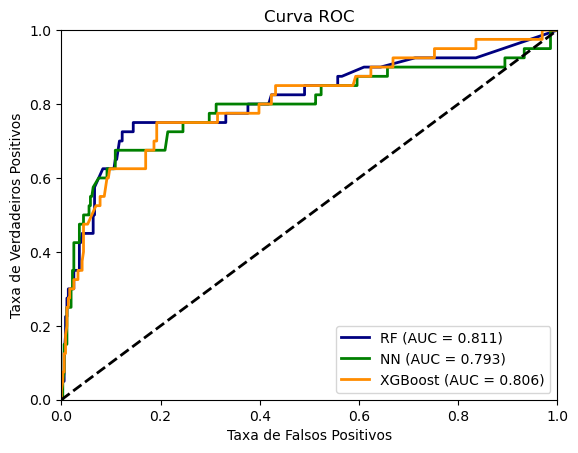
\includegraphics[width=.48\textwidth]{petrolesoeg100.png}
  \caption{Curva ROC de classificadores treinados com dados obtidos dos textos longos através de do petrolês O\&G 100}
  \label{fig:petrolesoeg100}
  \end{figure}

  \begin{figure}[ht]
  \centering
  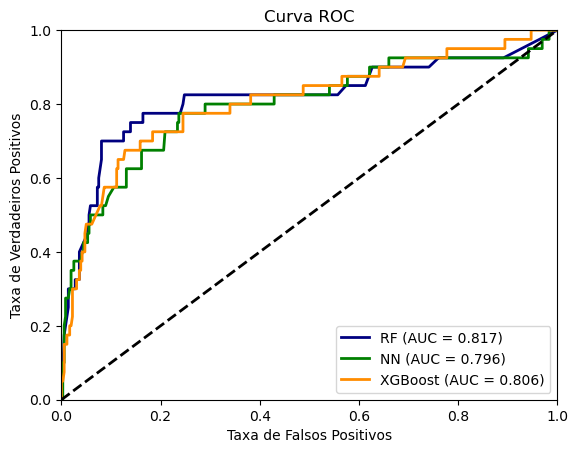
\includegraphics[width=.48\textwidth]{petrolesoeg100-sm.png}
  \caption{Curva ROC de classificadores treinados com dados obtidos dos textos longos através de do petrolês O\&G 100 e com data augmentation usando SMOTE}
  \label{fig:petrolesoeg100-sm}
  \end{figure}

  Os resultados obtidos mostram que é possível obter desempenho competitivo com técnicas consolidadas, simples e que rodam localmente, eliminando os custos e a dependência de um serviço fornecido através de uma API \cite{neelakantan2022text}.

    É possível observar dos resultados que ambos os modelos de \textit{embedding} aplicados conseguem se distanciar bastante de um classificador aleatório (linha tracejada preta) porém ainda estão distantes de um classificador perfeito. Ordens de manutenção são objetos que possuem, além do texto longo associado, diversas outras características relacionais (data de criação, data de encerramento, status, tipo, centro, entre outras). É provável que o uso da classificação por texto longo em conjunto com a classificação por essas características relacionais gere resultados ainda melhores.
    
\begin{table}
    \centering
    \caption{Tabela comparativa de diferentes técnicas de codificação}
    \label{tab:my_label}
    \def\arraystretch{1.2}
    \begin{tabular}{cccc} 
        \hline
        Técnica & Dimensões & Camadas & Parâmetros \\ 
        \hline
        TF-IDF & 1000 & -& -\\ 
        \hline
        GPT & 1536 & -& -\\ 
        \hline
        BERTimbau & 768 & 12 & 110 M \\ 
        \hline
        Petrolês 100 & 100 & -& -\\ 
        \hline
        Petrolês 300 & 300 & -& -\\ 
        \hline
        SBERT & 512 & -& -\\ 
        \hline
    \end{tabular}
\end{table}
  
\section{Conclusão}

  Foram encontradas diversas referências voltadas para a classificação automática de textos em português e os grandes modelos de linguagem possuem em suas bases de treinamento muitos conteúdos em português e, graças a isso, "falam" o idioma brasileiro com bastante fluência.
  Foi utilizada como referência de desempenho uma técnica tradicional de processamento de linguagem natura com a criação de uma matriz TF-IDF e posterior redução de dimensionalidade com SVD e treino de classificadores. Posteriormente foi realizado \textit{embedding} de sentenças com uma API da OpenAI e treino de um classificador similar ao do método anterior. Também foi realizado o \textit{embedding} com o SBERT e com o Petrolês. Finalmente foi realizado o embedding com o modelo BERTimbau \cite{souza2020bertimbau}. Os embeddings gerados pelo Petrolês apresentaram resultados competitivos com as vantagens de não depender do uso de uma API (cujo custo pode mudar, pode ser descontinuada, ou pode simplesmente estar indisponível devido à elevada demanda) e de não levar várias horas para rodar localmente (como foi observado com o BERTimbau)
  Considerando os fatores citados anteriormente, para a aplicação específica de classificação de textos longos de ordens de manutenção, é indicado o uso de um dos modelos treinados disponíveis no repositório do Petrolês.
  Trabalhos futuros podem avaliar o desempenho dessas técnicas aplicadas a um subconjunto diferente de ordens, assim como explorar melhor os hierparâmetros dos classificadores.

\section{Repositório}

  Códigos utilizados para a obtenção dos resultados se encontram disponíveis no seguinte repositório público do GitHub: https://github.com/ThomasAndarilho/AutoSAO/

\bibliographystyle{IEEEtran}
\bibliography{IEEEtran.bib}

\end{document}
